% Unofficial UofT Poster template.
% A fork of the UMich template https://www.overleaf.com/latex/templates/university-of-michigan-umich-poster-template/xpnqzzxwbjzc
% which is fork of the MSU template https://www.overleaf.com/latex/templates/an-unofficial-poster-template-for-michigan-state-university/wnymbgpxnnwd
% which is a fork of https://www.overleaf.com/latex/templates/an-unofficial-poster-template-for-new-york-university/krgqtqmzdqhg
% which is a fork of https://github.com/anishathalye/gemini
% also refer to https://github.com/k4rtik/uchicago-poster

\documentclass[final]{beamer}


% ====================
% Packages
% ====================
\usepackage[backend=biber, style=numeric, citestyle=numeric, sorting=none]{biblatex}\usepackage[T1]{fontenc}
 \usepackage[utf8]{luainputenc}
\usepackage{lmodern}
\usepackage{subfigure}
\usepackage[size=custom, width=122,height=91, scale=1.2]{beamerposter}
\usetheme{gemini}
\usecolortheme{uoft}
\usepackage{graphicx}
\usepackage{booktabs}
\usepackage{tikz}
\usepackage{pgfplots}
\pgfplotsset{compat=1.14}
\usepackage{anyfontsize}
\usepackage{tikz}
\usepackage{amsmath}
\usepackage{amssymb}
\usepackage{caption}
\usepackage{setspace}
\usepackage{wrapfig}
\usepackage{anyfontsize} % Allows custom font sizes
\usetikzlibrary{arrows.meta, positioning, shapes, fit, backgrounds}
\addbibresource{poster.bib}
\AtBeginBibliography{\tiny}

% ====================
% Lengths
% ====================

% If you have N columns, choose \sepwidth and \colwidth such that
% (N+1)*\sepwidth + N*\colwidth = \paperwidth
\newlength{\sepwidth}
\newlength{\colwidth}
\setlength{\sepwidth}{0.025\paperwidth}
\setlength{\colwidth}{0.3\paperwidth}

\newcommand{\separatorcolumn}{\begin{column}{\sepwidth}\end{column}}

% ====================
% Title
% ====================

\title{\huge Trump Tweets Before \& After 2021}

\author{
    Benedetta Gasbarra, Martin Ledesma, Tyler Nguyen, Ryo Sato, \\Mingye Wang, Richard Xu}

%\institute[shortinst]{University of California, Los Angeles}

% ====================
% Footer (optional)
% ====================



% (can be left out to remove footer)

% ====================
% Logo (optional)
% ====================

% use this to include logos on the left and/or right side of the header:
% Left: institution
 \logoright{
\includegraphics[height=10cm]{logos/image-removebg-preview (4).png}}
 \logoleft{
\includegraphics[height=6cm]{logos/stats logo.png}}
% Right: funding agencies and other affilations 
%\logoright{\includegraphics[height=7cm]{logos/NSF.eps}}

% ====================
% Body
% ====================

\begin{document}



\begin{frame}[t]
\begin{columns}[t]
\separatorcolumn
\begin{column}{\colwidth}

  \begin{block}{Goal}
    Our goal is to analyze various aspects of former President Donald Trump's tweets given his particular influence on American politics. We aim to examine:
    \vspace{-15pt}
    \begin{itemize}
        \item His frequency of tweets over different time periods.
        \item His flagged versus non-flagged tweet favorite counts.
        \item His average tweet length between flagged and non-flagged tweets.
    \end{itemize}
    \vspace{-15pt}
    Additionally, we will apply text-based analysis to develop a model that estimates the probability of Trump's post-2021 tweets being flagged, based on patterns observed in his pre-2021 tweets. This analysis is conducted within the context of Elon Musk's acquisition of Twitter and Trump's subsequent unbanning.
  \end{block}
 \vspace{-15pt}
  \begin{block}{Exploratory Data Analysis \& Hypothesis Testing}
  Using our visualizations from Exploratory Data Analysis, we are able to draw some hypotheses and test them:
  \vspace{-15pt}
  \begin{itemize}
            \item \textbf{Hypothesis 1:}
            \begin{itemize}
                    \item[] $H_0$: Number of tweet frequency doesn’t go up during election season.
                    \item[] $H_a$: Number of tweet frequency goes up during election season.
                \end{itemize}
                \begin{figure}
                    \centering
                    \hfill
                    \subfigure[Number of tweets over time BEFORE BAN]{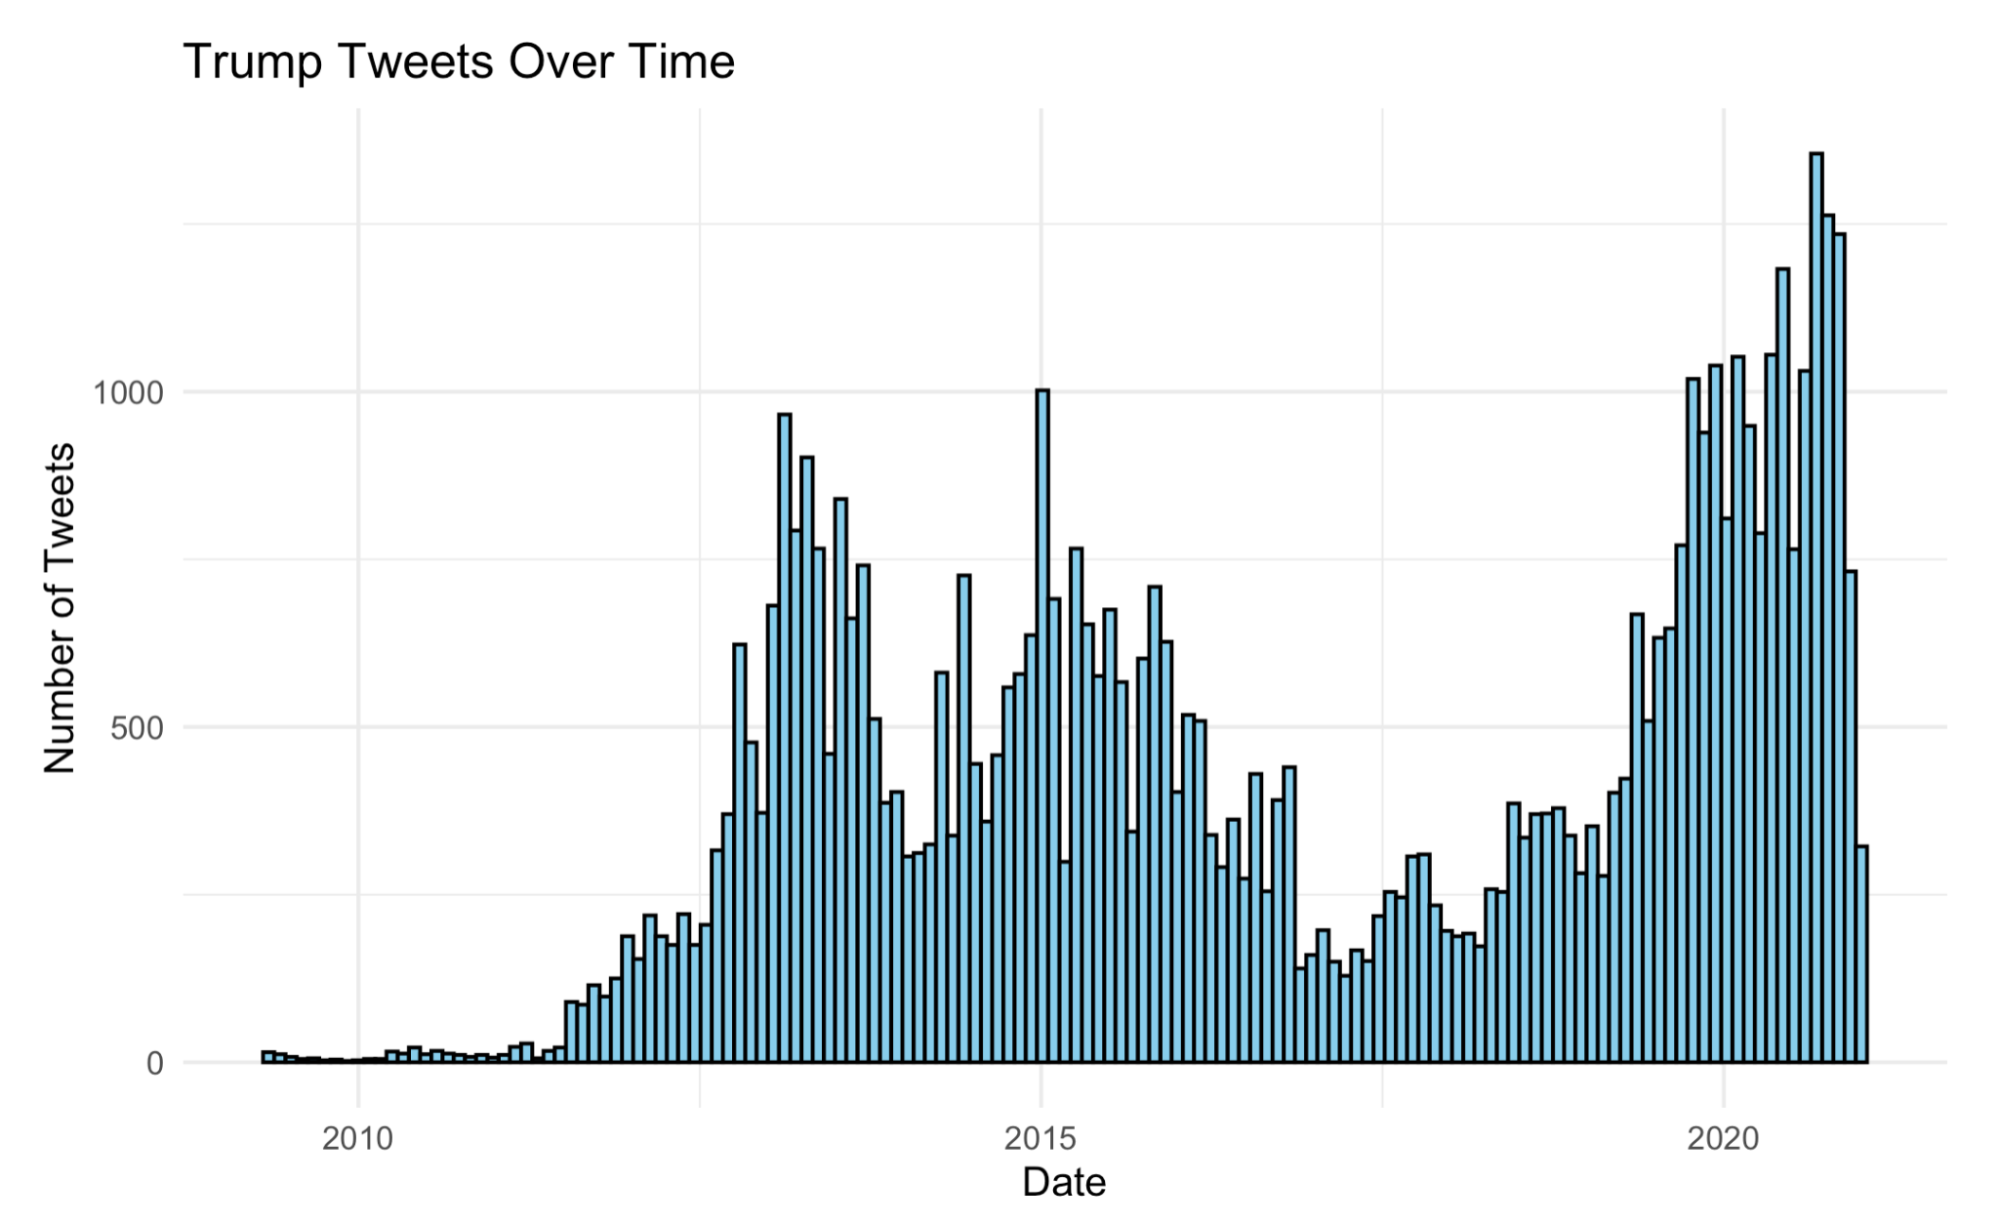
\includegraphics[width=17cm]{figures/TweetsOvertimeBefore.png}}
                    \hfill
                    \subfigure[Number of tweets over time AFTER BAN]{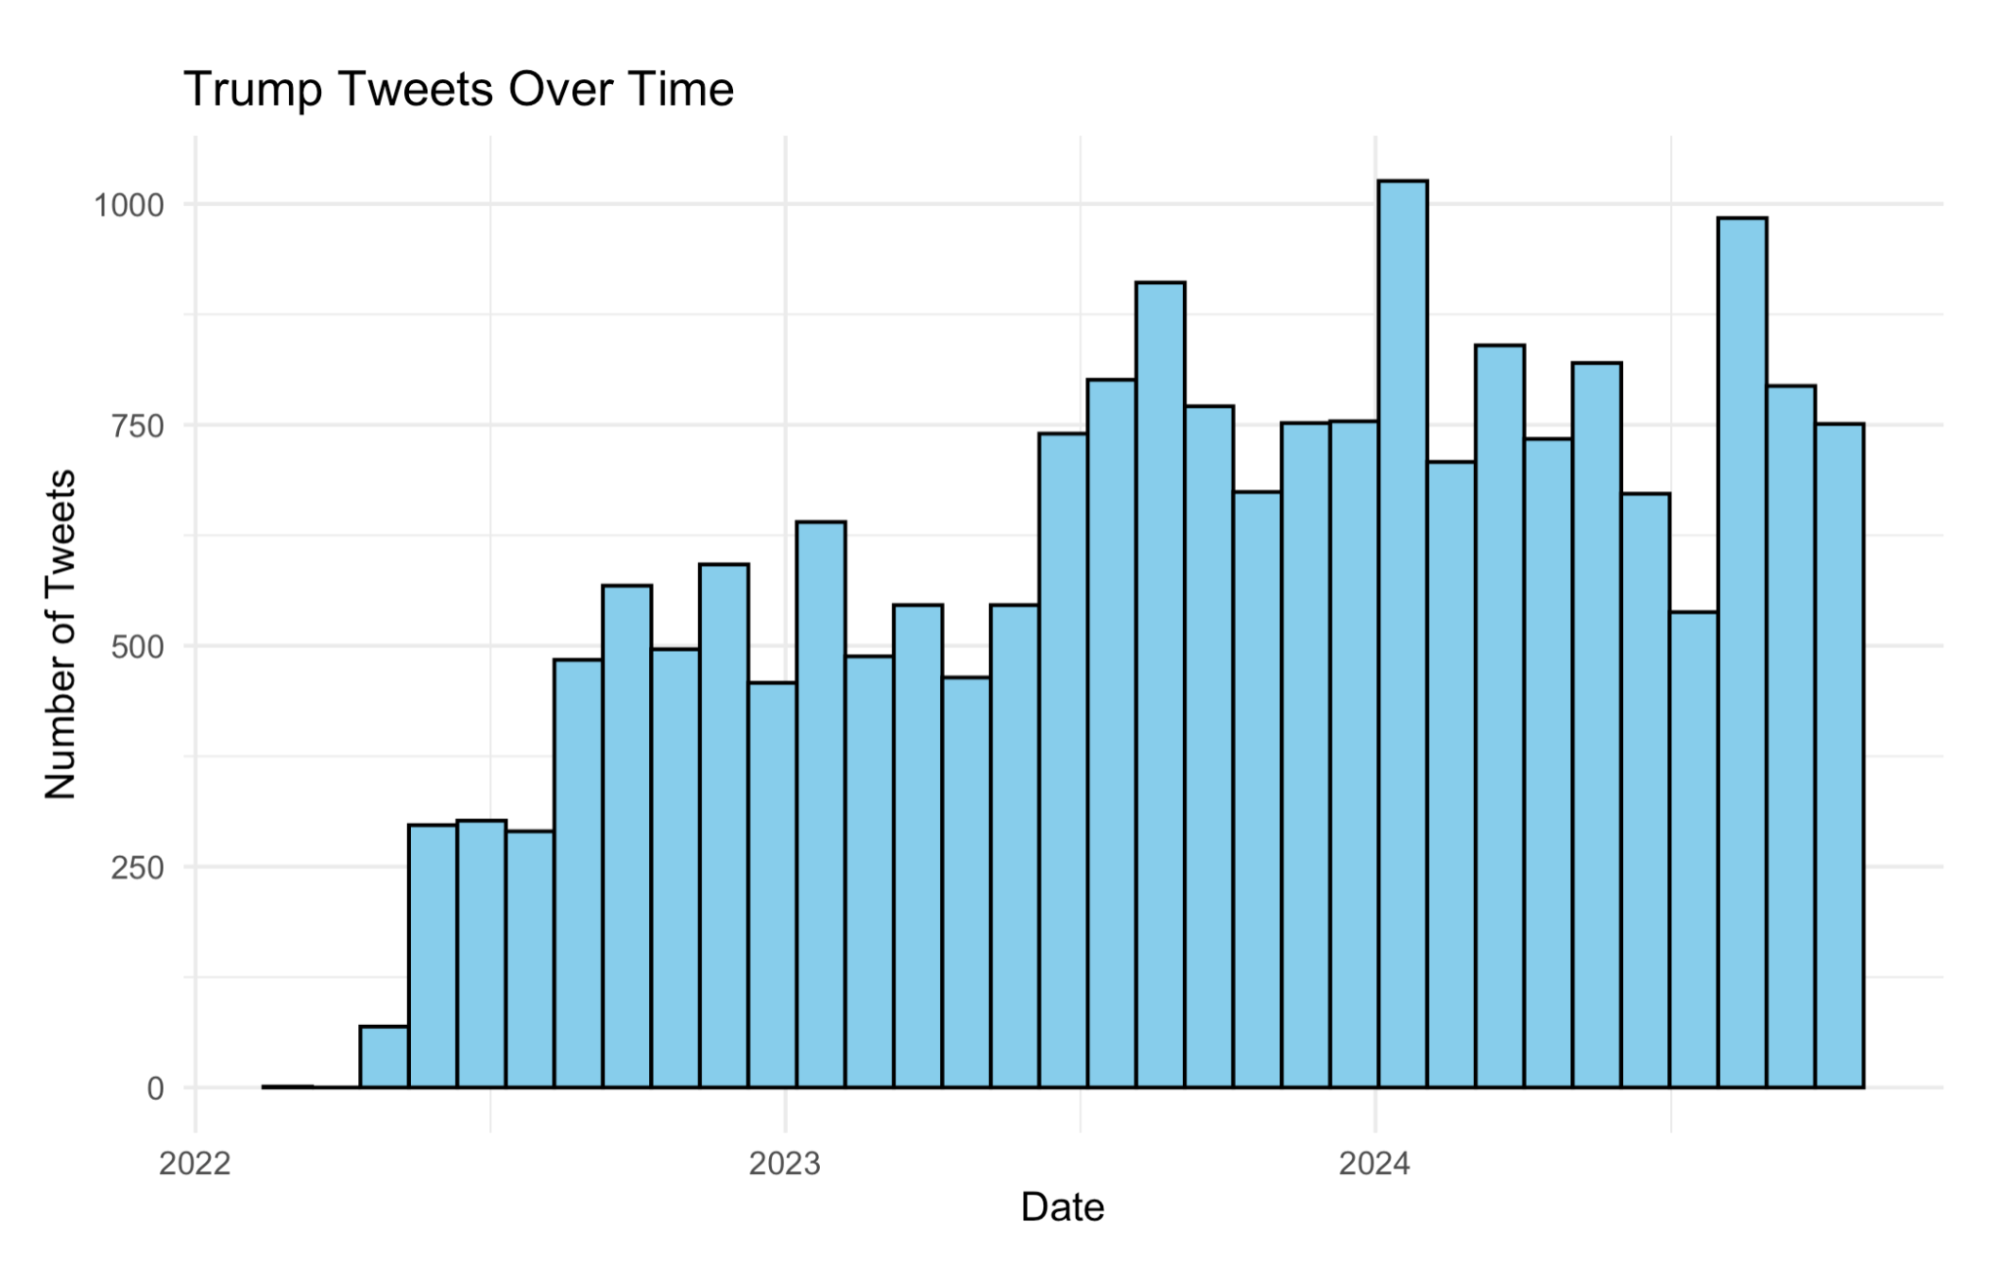
\includegraphics[width=17cm]{figures/TweetsOvertimeAfter.png}}
                \end{figure}
        The two histograms show that Trump tends to tweet more frequently around election season. A Welch's Two-Sample t-test confirmed this with a significant p-value, supporting Trump tweets more during election season.
            \item \textbf{Hypothesis 2:}
                \begin{itemize}
                    \item[] $H_0$: The distribution of favorites is the same for flagged and non-flagged tweets.
                    \item[] $H_a$: Trump's flagged tweets have more favorites than non-flagged tweets.
                \end{itemize}
                \begin{figure}
                        \centering
                        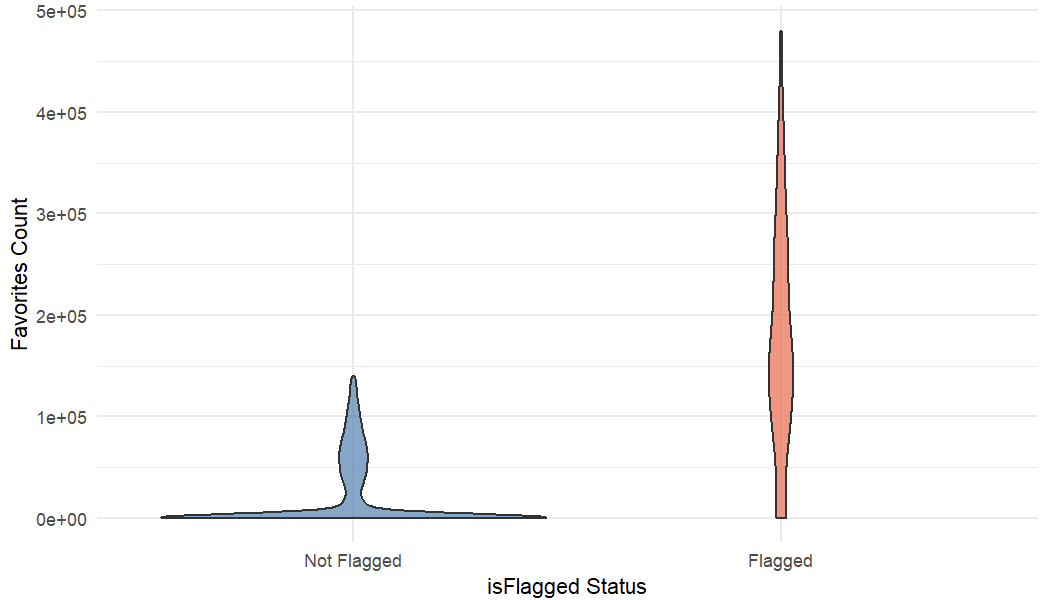
\includegraphics[width=0.9\textwidth]{figures/favoritesviolincrop.png}
                        \caption{Comparison of Favorites Count between Flagged \& Non-Flagged Tweets.}
                    \end{figure}
        \end{itemize}
        The violin plot shows that flagged tweets have a wider range and higher favorite counts compared to non-flagged tweets. A Wilcoxon signed-rank test confirmed this with a significant p-value, supporting the conclusion that flagged tweets generally receive more favorites.

    \begin{itemize}
    \begin{large}
    \end{large}
  \end{itemize}
% we should use figures that discuss the hypothesis we want to talk about
% \begin{figure}
%     \centering
%     \hfill
%     \subfigure[Number of tweets over time BEFORE BAN]{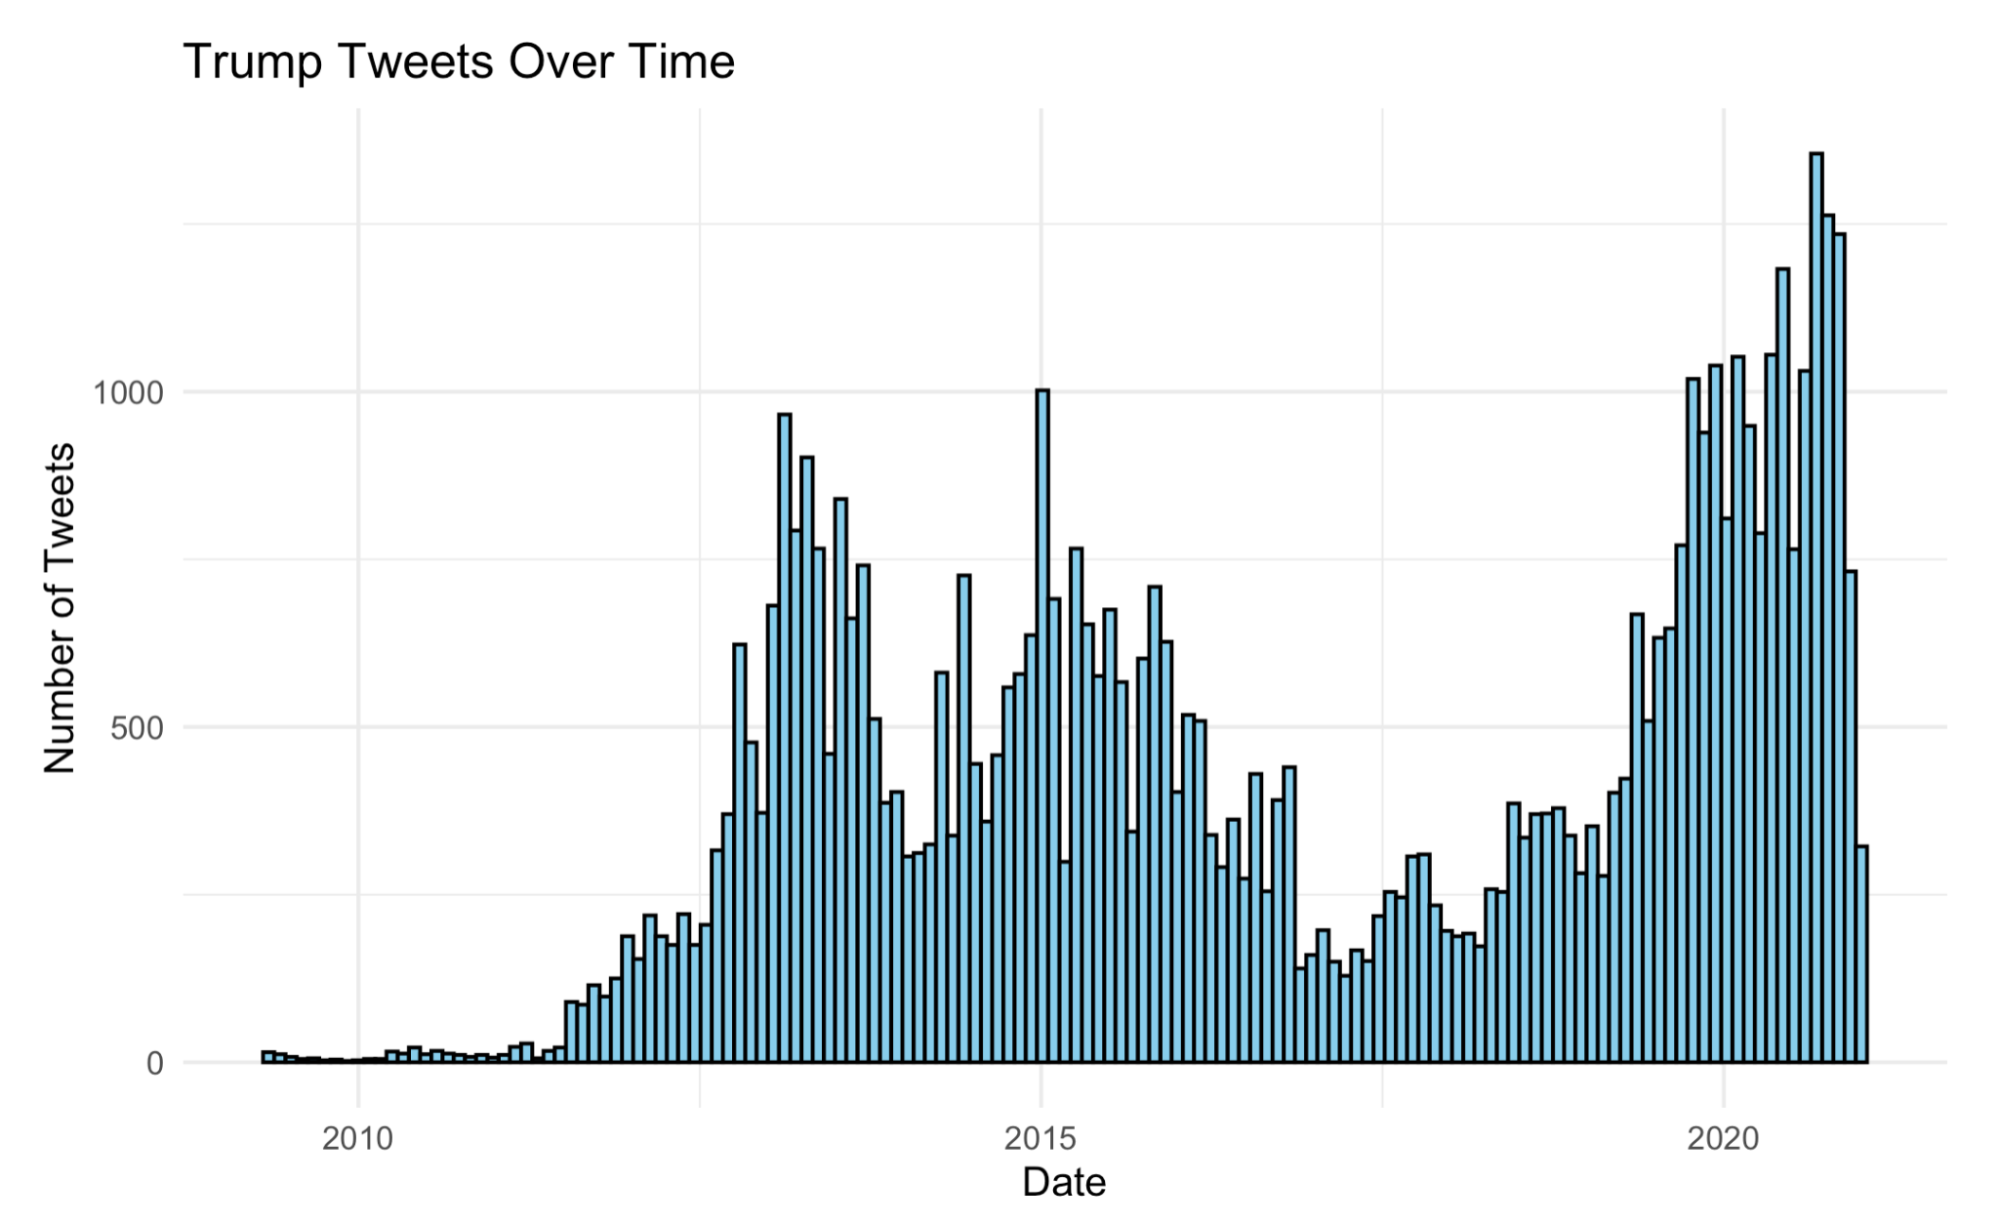
\includegraphics[width=17cm]{figures/TweetsOvertimeBefore.png}}
%     \hfill
%     \subfigure[Number of tweets over time AFTER BAN]{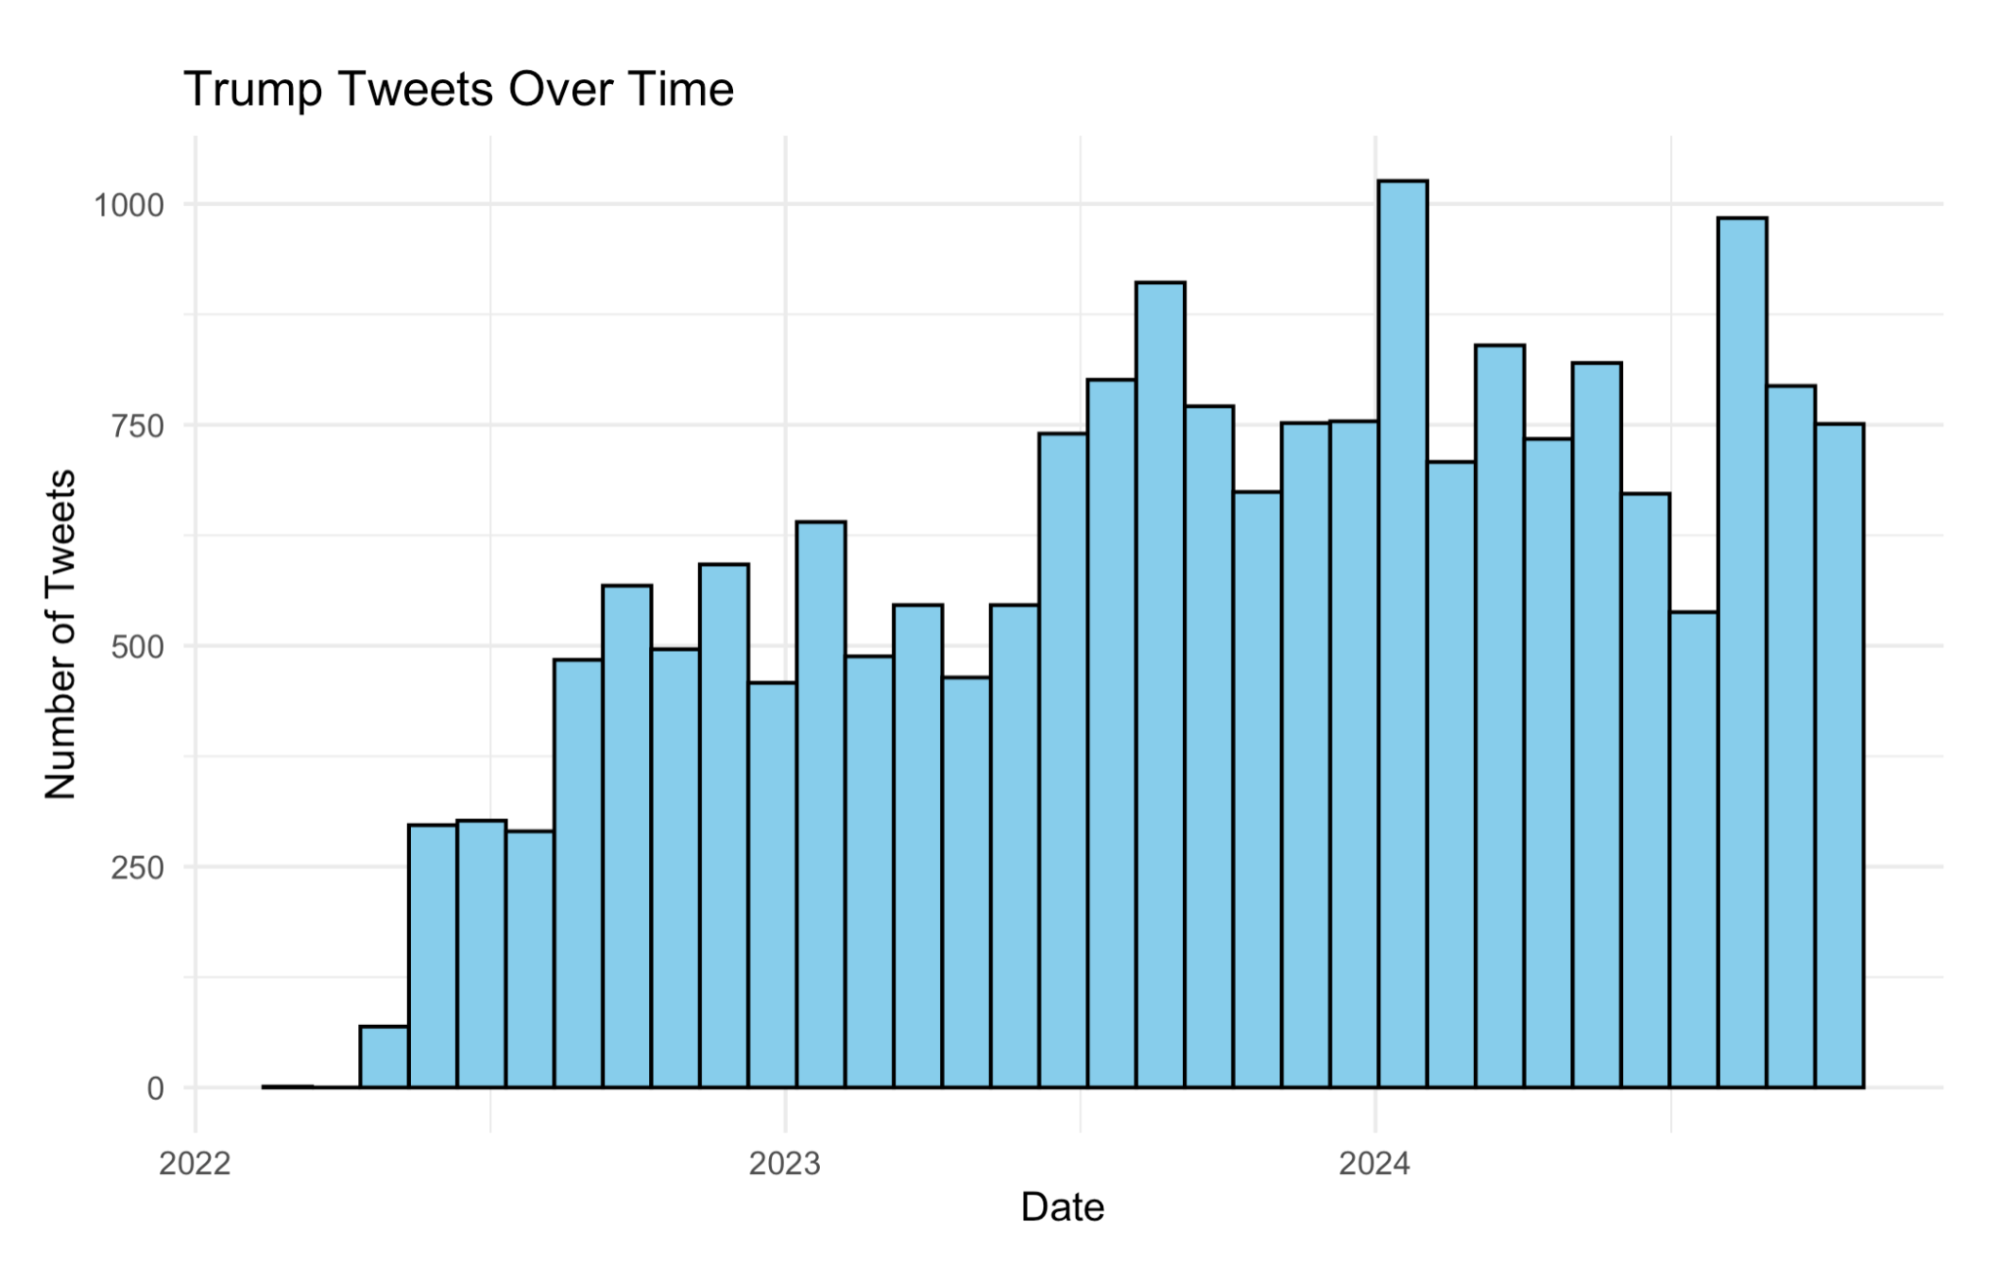
\includegraphics[width=17cm]{figures/TweetsOvertimeAfter.png}}
%     \hfill

%     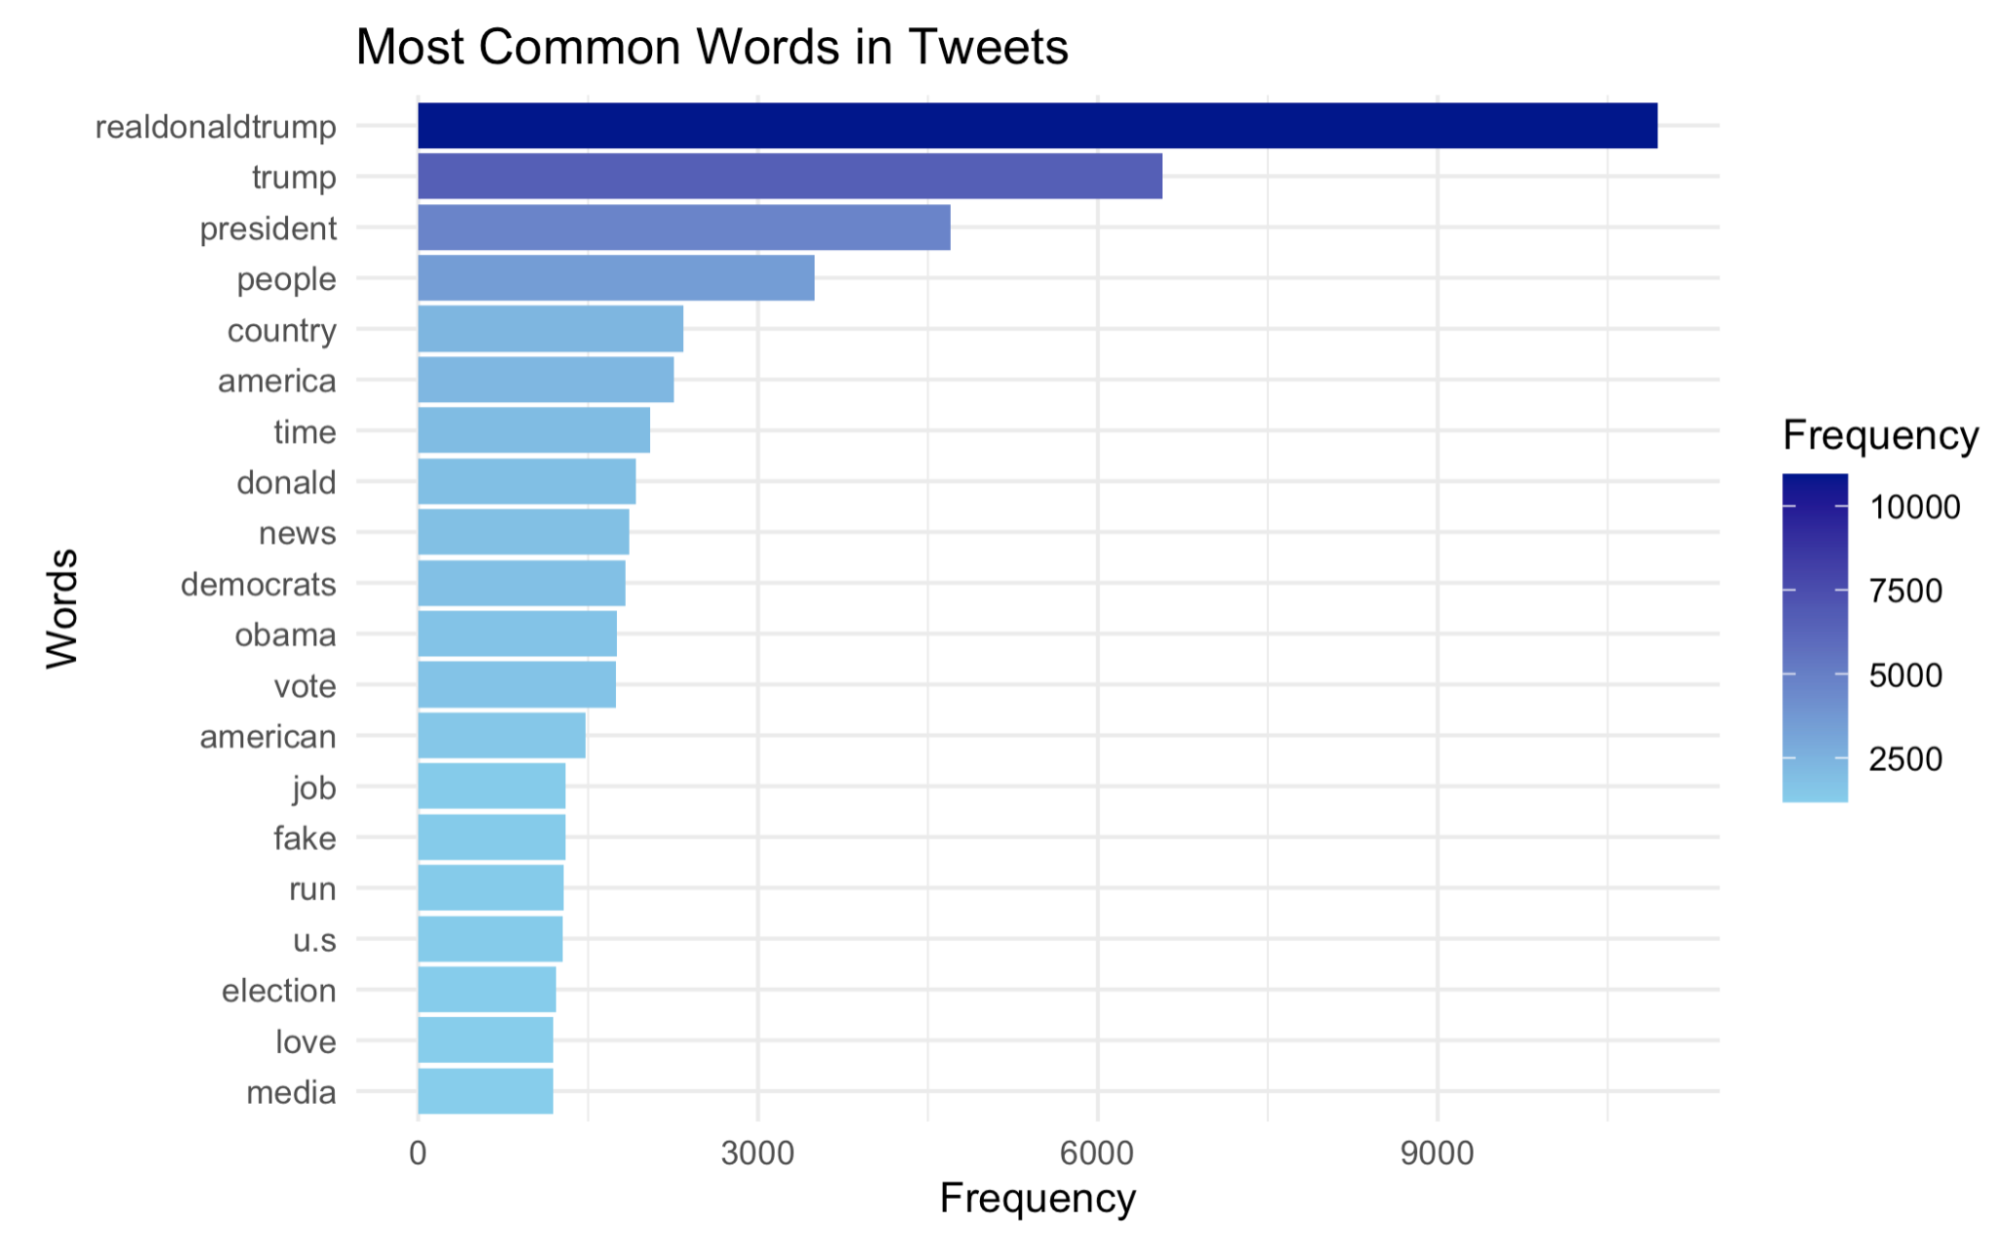
\includegraphics[scale = 0.35]{figures/PopularWords.png}
        
%     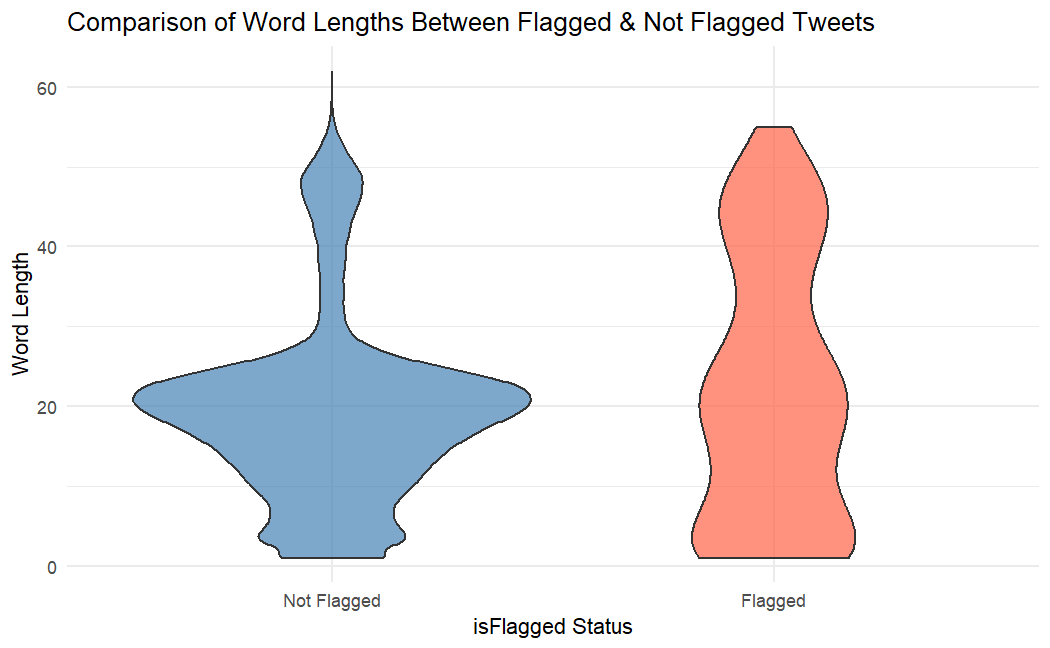
\includegraphics[width = 30cm]{figures/newviolin.png}
%     \end{figure}
\end{block}

\end{column}

\separatorcolumn

\begin{column}{\colwidth}
    \begin{block}{Hypothesis Testing (Continued)}
    \begin{itemize}
        \item \textbf{Hypothesis 3:}
            \begin{itemize}
                    \item[] $H_0$: Trump’s pre-2021 flagged tweets are not longer than his normal tweets.
                    \item[] $H_a$: Trump’s pre-2021 flagged tweets are longer than his normal tweets.
            \end{itemize}
                    \begin{figure}
                        \centering
                        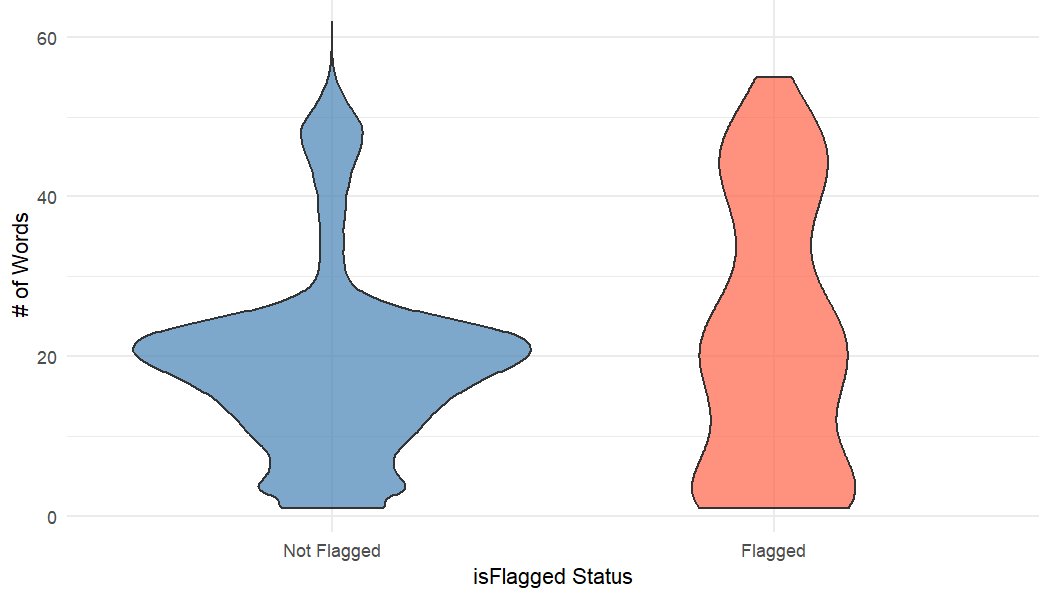
\includegraphics[width=0.75\textwidth]{figures/violinplotnotitle.png}
                        \caption{Comparison of Word Count between Flagged \& Non-Flagged Tweets.}
                    \end{figure}
    \end{itemize}
    The violin plot shows that flagged tweets tend to have more words compared to non-flagged tweets. A Welch's Two-Sample t-test confirmed this with a significant p-value, supporting the conclusion that flagged tweets are generally longer.
    \end{block}
    \vspace{-30pt}  % Reduces space, adjust as necessary
    \begin{block}{Classification Model}
        In our modeling, we had to account for the textual nature of the data and the imbalanced Flagged to non-Flagged observations.

        To tackle the imbalance between Flagged and non-Flagged observations in our dataset, we applied sampling techniques such as oversampling, undersampling, and SMOTE.

        We then tested several models, including Logistic Regression, XGBoost, and Random Forest. However, all models struggled with high accuracy due to overtraining on non-Flagged data, while precision and recall for Flagged observations remained low.

        Adding sentiment analysis as a feature had minimal impact on performance. Ultimately, we opted for a simpler approach: TF-IDF (Term Frequency-Inverse Document Frequency). This method captures how often terms appear in tweets while accounting for their overall frequency across the dataset, delivering similar results to the more complex models.
        \vspace{-30pt}
        \begin{figure}
            \centering
            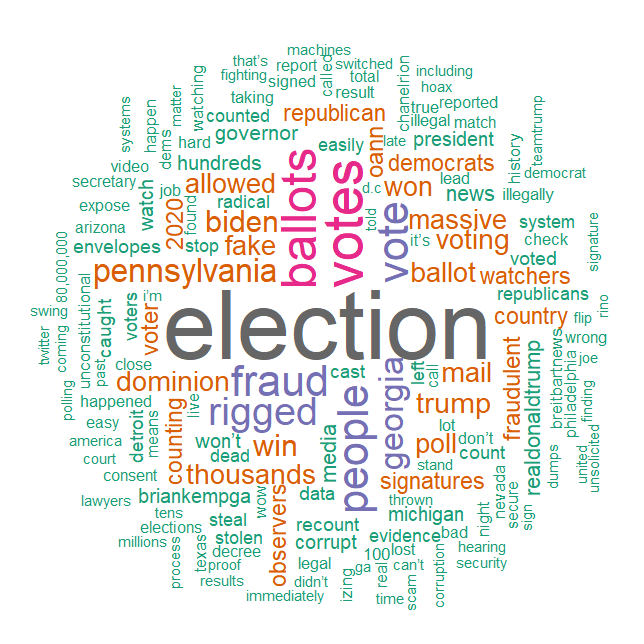
\includegraphics[scale=1.22]{figures/wordcloud.png}
            \caption{Trump's Favorite Flagged Words} 
        \end{figure}

 
    \begin{large}

    \end{large}
\vspace*{-5mm}
\begin{enumerate}

    \begin{large}
    
 
    
    \end{large}   
\end{enumerate}



  \end{block}
    

\end{column}

\separatorcolumn

\begin{column}{\colwidth}

    \begin{block}{Algorithm}
        We separated the dataset based on the isFlagged status, applying TF-IDF to each subset. The parameters were set to extract a maximum of 3,000 features, with each feature being a unigrams, bigrams, or trigrams (1–3 words in length). For instance, phrases like "rigged election" were identified as significant features. This process generated weighted representations of words and phrases specific to both flagged and non-flagged data. By comparing the two sets, we identified the terms present in the flagged set but absent from the non-flagged set. 
        \begin{figure}
            \centering
            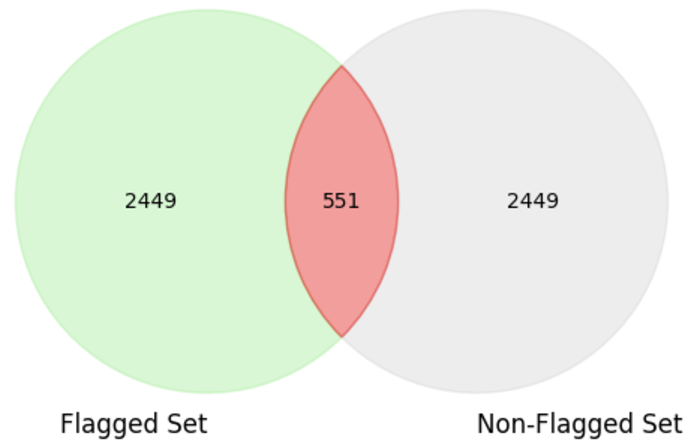
\includegraphics[scale=0.9]{figures/venndiagram.png}
            \caption{We keep the green and remove the red overlap.}
        \end{figure}
        These distinctive words and phrases were then used to classify tweets as flagged or non-flagged.
    \end{block}
    \vspace*{-5mm}
    \begin{block}{Model Analysis}
        After running our model on the original dataset, we created a frequency table to show actual vs. prediction.
        \begin{table}[h!]
            \centering
            \begin{tabular}{|c|c|c|}
                \hline
                \textbf{} & \textbf{Predicted: No Flag} & \textbf{Predicted: Flag} \\
                \hline
                \textbf{Actual: No Flag} & 53,677 & 2,590 \\
                \hline
                \textbf{Actual: Flag} & 120 & 184 \\
                \hline
        \end{tabular}
\caption{Confusion Matrix}
\end{table}
        \vspace*{-15pt}
        \textbf{\emph{Model Performance Summary:}}
        \vspace*{-15pt}
        \begin{itemize}
            \item \textbf{Accuracy:} \emph{95.48\%} of total predictions were correct, indicating a high overall prediction rate.
            \item \textbf{True Positives (Flagged Tweets):} Only \emph{6.63\%} of the flagged tweets were correctly identified as positive by the model.
            \item \textbf{Recall:} The model successfully identifies \emph{60.53\%} of the actual flagged tweets.
            \item \textbf{F1 Score:} The low F1 score of \emph{11.91\%} suggests that while the model detects some flagged tweets, it also produces many incorrect predictions.
        \end{itemize}
        \vspace*{-15pt}
        Though these are not the best results, they are comparable to other complicated models applied to the training data.
    \end{block}
\vspace*{-15pt}
  \begin{block}{Conclusions}
    When applied to post-2021 data, our model predicted \textbf{17,305 non-flagged tweets and 2,206 flagged tweets}. While these results align with our current efforts, the model is not the optimal solution given the constraints of time and resources.
    
    In future iterations, we would prioritize addressing sample imbalance through improved sampling methods and explore more computationally intensive models to better capture nuanced patterns in the tweets.

    It would also be nice to implement the Topic Models that we did come up with but did not have the time to use.
    
  \begin{large}
\begin{itemize}

\end{itemize}
\end{large}
\end{block}

\end{column}


\separatorcolumn
\end{columns}

\end{frame}

\end{document}
